\section{Problem description}


% \begin{itemize}
%     \item Maxime \ok ? \no ?
%     \item Thierry \ok ? \no ?
%     \item Victor \ok ? \no ?
% \end{itemize}

In this section we present the  problems encountered with using one hot encoding and then illustrate it in the online learning set up.


\subsection{Notation}\label{notations}

We consider the supervised learning set up with a given set of training labeled data $\mathcal{Z} = \{ z_i = (X_i; y_i); i = 1 \dots  n \}$, with the feature
vectors $X_i \in \mathbb{R}^p$ and the scalar targets $y_i \in \mathbb{R}$. Each one of the $p$ components of the feature vectors is related to one of the $p$ symbols $\{ s_k\}_{k \leq p}$:

\begin{equation} \label{eq:symbol}
    \forall (X_i, \cdot) \in \mathcal{Z} \quad \forall k \leq p \quad X_i \text{ corresponds to } s_k \iif X_{i}^k \neq 0
\end{equation}

We aim to find the best parameter $\theta^\star \in \mathbb{R}^m$ ($m \geq p$) to minimize the loss $F_{\theta^\star}$ on the whole dataset:

\begin{align*}
    f: \quad &\Theta \times \mathcal{Z} \longrightarrow \mathbb{R}\\
            &\theta, (X,y) \longrightarrow  f_{\theta}(X,y)
\end{align*}

\begin{align*}
\theta^\star &= \underset{\theta}{\argmin} \quad F_\theta\\
             &= \underset{\theta}{\argmin} \sum_{X,y \in \mathcal{Z}} f_\theta (X,y)\\
             &= \underset{\theta}{\argmin} \sum_{i=1\dots n} f_\theta (X_i,y_i)
\end{align*}

This notation is generic and includes sparse data in general. One-hot encoded data is a specific case of sparse data.














%%%%%%%%%%%%%%%%%%%%%%%%%%%%%%%%%%%%%%%%%%%%%%%%%%%%%%%%%%%%%%%%%%%%%%%%%%%%%%%%%%%%%%%%%
%%%%%%%%%%%%%%%%%%%%%%%%%%%%%%%%%%%%%%%%%%%%%%%%%%%%%%%%%%%%%%%%%%%%%%%%%%%%%%%%%%%%%%%%%
%%%%%%%%%%%%%%%%%%%%%%%%%%%%%%%%%%%%%%%%%%%%%%%%%%%%%%%%%%%%%%%%%%%%%%%%%%%%%%%%%%%%%%%%%
%%%%%%%%%%%%%%%%%%%%%%%%%%%%%%%%%%%%%%%%%%%%%%%%%%%%%%%%%%%%%%%%%%%%%%%%%%%%%%%%%%%%%%%%%
%%%%%%%%%%%%%%%%%%%%%%%%%%%%%%%%%%%%%%%%%%%%%%%%%%%%%%%%%%%%%%%%%%%%%%%%%%%%%%%%%%%%%%%%%
%%%%%%%%%%%%%%%%%%%%%%%%%%%%%%%%%%%%%%%%%%%%%%%%%%%%%%%%%%%%%%%%%%%%%%%%%%%%%%%%%%%%%%%%%
%%%%%%%%%%%%%%%%%%%%%%%%%%%%%%%%%%%%%%%%%%%%%%%%%%%%%%%%%%%%%%%%%%%%%%%%%%%%%%%%%%%%%%%%%

\begin{figure*}
\centering
\begin{subfigure}{0.48\linewidth}
\centering
%%\begin{figure}[h!]
%%\centering
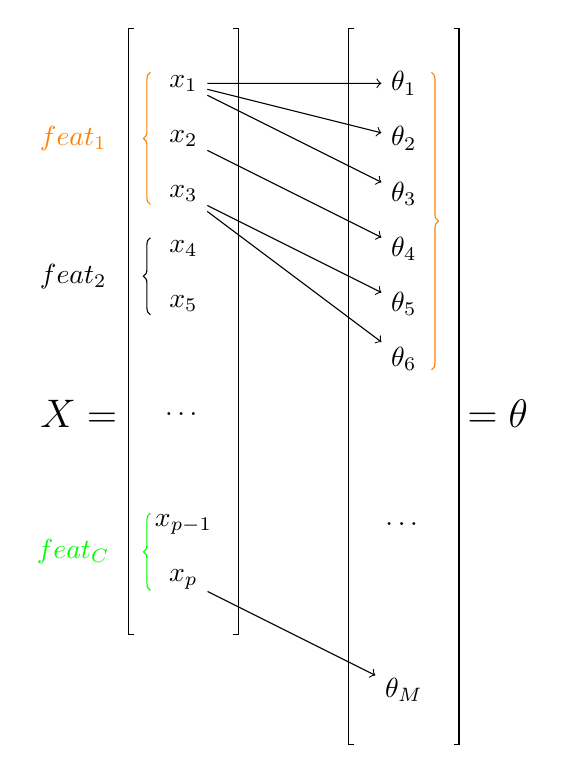
\begin{tikzpicture}[scale=0.7]

\draw (-0.9,11) --(-1,11) -- (-1,0) -- (-0.9,0) ;
\draw (0.9,11) --(1,11) -- (1,0) -- (0.9,0) ;

\node (x1)   at (0,10)  {$x_1$};
\node (x2)   at (0,9)  {$x_2$};
\node (x3)   at (0,8)  {$x_3$};
\node (x4)   at (0,7)  {$x_4$};
\node (x5)   at (0,6)  {$x_5$};
\node (xdot) at (0,4)  {\dots};
\node (xpm1) at (0,2)  {$x_{p-1}$};
\node (xp)   at (0,1)  {$x_p$};

\node (feat1) at (-2,9)   {\textcolor{orange}{$feat_1$}};
\node (feat2) at (-2,6.5) {\textcolor{black}{$feat_2$}};
\node (feat3) at (-2,1.5) {\textcolor{green}{$feat_C$}};



\node (X)     at (-1.9,4) {\Large $X = $};
\node (Theta) at (5.7,4)  {\Large $ = \theta $};


\draw [decorate, decoration = {brace,mirror}, color=orange] (-0.6,10.2) -- (-0.6,7.8);
\draw [decorate, decoration = {brace,mirror}, color=black]  (-0.6,7.2)  -- (-0.6,5.8);
\draw [decorate, decoration = {brace,mirror}, color=green]  (-0.6,2.2)  -- (-0.6,0.8);


\draw (3.1,11) --(3,11) -- (3,-2) -- (3.1,-2) ;
\draw (4.9,11) --(5,11) -- (5,-2) -- (4.9,-2) ;

\node (theta1)   at (4,10)   {$\theta_1$};
\node (theta2)   at (4,9)    {$\theta_2$};
\node (theta3)   at (4,8)    {$\theta_3$};
\node (theta4)   at (4,7)    {$\theta_4$};
\node (theta5)   at (4,6)    {$\theta_5$};
\node (theta6)   at (4,5)    {$\theta_6$};
\node (thetadot) at (4,2)    {\dots};
\node (thetaM)   at (4,-1)  {$\theta_M$};


\path [->] (x1) edge[draw=black] (theta1);
\path [->] (x1) edge[draw=black] (theta2);
\path [->] (x1) edge[draw=black] (theta3);
\path [->] (x2) edge[draw=black] (theta4);
\path [->] (x3) edge[draw=black] (theta5);
\path [->] (x3) edge[draw=black] (theta6);
\path [->] (xp) edge[draw=black] (thetaM);

\draw [decorate, decoration = {brace,mirror}, color=orange]  (4.5,4.8) -- (4.5,10.2) ;

\end{tikzpicture}
\caption{Generic n  otations}
\label{fig:generalnotations}
\end{subfigure}
\begin{subfigure}{0.48\linewidth}

%%\begin{figure}[h!]
%%\centering
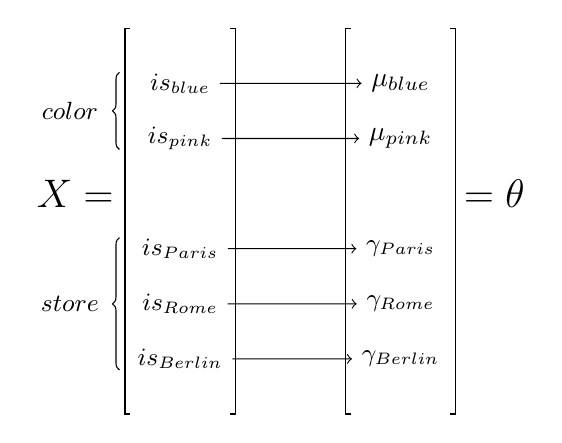
\begin{tikzpicture}[scale=0.7]

\draw (-0.9,11) --(-1,11) -- (-1,4) -- (-0.9,4) ;
\draw (0.9,11) --(1,11) -- (1,4) -- (0.9,4) ;

\node (blue)  at (0,10) {\small $is_{blue}$};
\node (pink)  at (0,9)  {\small $is_{pink}$};
\node (Paris)     at (0,7)  {\small $is_{Paris}$};
\node (Rome)     at (0,6)  {\small $is_{Rome}$};
\node (Berlin)     at (0,5)  {\small $is_{Berlin}$};

\node (color) at (-2,9.5)   {\small $color$};
\node (store) at (-2,6) {\small $store$};


\node (X)     at (-1.9,8) {\Large $X = $};
\node (Theta) at (5.7,8)  {\Large $ = \theta $};


\draw [decorate, decoration = {brace,mirror}] (-1.1,10.2) -- (-1.1,8.8);
\draw [decorate, decoration = {brace,mirror}] (-1.1,7.2) -- (-1.1,4.8);


\draw (3.1,11) --(3,11) -- (3,4) -- (3.1,4) ;
\draw (4.9,11) --(5,11) -- (5,4) -- (4.9,4) ;

\node (mublue)   at (4,10)   {$\mu_{blue}$};
\node (mupink)   at (4,9)    {$\mu_{pink}$};

\node (muparis)  at (4,7)    {\small $\gamma_{Paris}$};
\node (murome)   at (4,6)    {\small $\gamma_{Rome}$};
\node (muberlin) at (4,5)    {\small $\gamma_{Berlin}$};


\path [->] (blue)   edge[draw=black] (mublue);
\path [->] (pink)   edge[draw=black] (mupink);
\path [->] (Paris)  edge[draw=black] (muparis);
\path [->] (Rome)   edge[draw=black] (murome);
\path [->] (Berlin) edge[draw=black] (muberlin);


\end{tikzpicture}
\caption{Notations applied to Model \ref{catModel}}
\label{fig:notationsModel1}
\end{subfigure}
\caption{Notations}
\label{fig:notations}
\end{figure*}


Figure \ref{notations} illustrates the formal definition. In Figure \ref{fig:generalnotations}, $\{ \theta_1 ;  \theta_2 ;  \theta_3 ;  \theta_4 ;  \theta_5 ;  \theta_6 ; \}$ are related to the first feature $\textcolor{orange}{feat_1}$. On Model \ref{catModel}, such notations give Figure \ref{fig:notationsModel1}.
%%%%%%%%%%%%%%%%%%%%%%%%%%%%%%%%%%%%%%%%%%%%%%%%%%%%%%%%%%%%%%%%%%%%%%%%%%%%%%%%%%%%%%%%%
%%%%%%%%%%%%%%%%%%%%%%%%%%%%%%%%%%%%%%%%%%%%%%%%%%%%%%%%%%%%%%%%%%%%%%%%%%%%%%%%%%%%%%%%%
%%%%%%%%%%%%%%%%%%%%%%%%%%%%%%%%%%%%%%%%%%%%%%%%%%%%%%%%%%%%%%%%%%%%%%%%%%%%%%%%%%%%%%%%%
%%%%%%%%%%%%%%%%%%%%%%%%%%%%%%%%%%%%%%%%%%%%%%%%%%%%%%%%%%%%%%%%%%%%%%%%%%%%%%%%%%%%%%%%%
%%%%%%%%%%%%%%%%%%%%%%%%%%%%%%%%%%%%%%%%%%%%%%%%%%%%%%%%%%%%%%%%%%%%%%%%%%%%%%%%%%%%%%%%%
%%%%%%%%%%%%%%%%%%%%%%%%%%%%%%%%%%%%%%%%%%%%%%%%%%%%%%%%%%%%%%%%%%%%%%%%%%%%%%%%%%%%%%%%%
%%%%%%%%%%%%%%%%%%%%%%%%%%%%%%%%%%%%%%%%%%%%%%%%%%%%%%%%%%%%%%%%%%%%%%%%%%%%%%%%%%%%%%%%%
%%%%%%%%%%%%%%%%%%%%%%%%%%%%%%%%%%%%%%%%%%%%%%%%%%%%%%%%%%%%%%%%%%%%%%%%%%%%%%%%%%%%%%%%%
%%%%%%%%%%%%%%%%%%%%%%%%%%%%%%%%%%%%%%%%%%%%%%%%%%%%%%%%%%%%%%%%%%%%%%%%%%%%%%%%%%%%%%%%%
%%%%%%%%%%%%%%%%%%%%%%%%%%%%%%%%%%%%%%%%%%%%%%%%%%%%%%%%%%%%%%%%%%%%%%%%%%%%%%%%%%%%%%%%%
%%%%%%%%%%%%%%%%%%%%%%%%%%%%%%%%%%%%%%%%%%%%%%%%%%%%%%%%%%%%%%%%%%%%%%%%%%%%%%%%%%%%%%%%%
%%%%%%%%%%%%%%%%%%%%%%%%%%%%%%%%%%%%%%%%%%%%%%%%%%%%%%%%%%%%%%%%%%%%%%%%%%%%%%%%%%%%%%%%%
%%%%%%%%%%%%%%%%%%%%%%%%%%%%%%%%%%%%%%%%%%%%%%%%%%%%%%%%%%%%%%%%%%%%%%%%%%%%%%%%%%%%%%%%%




\subsection{Gradient descent with symbolic variables}\label{sec:motication}
Classical stochastic gradient descent relies on an unbiased gradient's estimator. Rather than using the complete gradient on all observations, observations are divided into \textit{batches} and the gradient is estimated on those:
\begin{align}
\nabla F &=  \frac{1}{n} \sum_{obs} \nabla f_{obs}  = \frac{1}{n} \sum_{i \leq n} \nabla_{\theta} f(X_i, y_i)     \\
         &= \frac{1}{n} \sum_{batch} \quad \sum_{obs \in batch} \nabla f_{obs}
\end{align}
In particular, this makes sense on large datasets where computing the exact full (i.e. on all observations) gradient might be very expensive.
The accumulated gradient is then divided by the size of the batch to get the gradient mean. Gradient descent techniques succeed in finding a minimum, notably because this the gradient estimator is unbiased. 

Regarding \catmod, we can highlight the fact that not every symbolic parameter is affected by every observation. For example in model \ref{catModel} $\mu_{blue}$ is only used on observations that concern a blue product. By construction via \ohe each observation concerns one and only one symbol for each symbolic feature. Applying Gradient descent in a batch mode to estimate the gradient gives a biased estimator. This issue is exacerbated on a batch that does not include a symbol. In this instance, the gradient does not even make sense.

\begin{align}
\nabla_{\mu_{blue}} F &= \frac{1}{n} \sum_{obs} \nabla_{\mu_{blue}} f_{obs}\\
         &= \frac{1}{n} \sum_{batch} \underset{color(obs) = blue}{\sum_{{obs \in batch}}} \nabla_{\mu_{blue}} f_{obs}
\label{eq:gradientDecomp}
\end{align}


What would be the parameter's gradient of a symbol that is not present at all in the dataset? What would be the gradient of $\mu_{red}$ in Model \ref{catModel} with no red products? $\{ obs \in batch | color(obs) = blue \}$ from Equation \ref{eq:gradientDecomp} might be empty, and in this case parameters related to the \textit{blue} symbol are not present. And \mainContrib. Thanks to \ohe, we have prior info on the data and the gradient. With an observation that does not concerns the symbol $s_k$, we know \textbf{for a fact} that the gradient of its related parameters will be numerically zero. Thus this numerically zero gradient does not bring any information, it should not be used for parameters updates.

\begin{align*}
    &\mu_{color} = \mu_{blue} \times is_{blue} + \mu_{pink} \times is_{pink} \numberthis \label{eq:muEncoding} \\
    &\frac{\partial\mu_{color}}{\partial\mu_{blue}}\mid_{color = pink} = 0\\
    &\frac{\partial\mu_{color}}{\partial\mu_{pink}}\mid_{color = blue} = 0
\end{align*}


This issue  especially concerns under-represented symbols and small batches. The smallest the symbol cardinality and the smallest the batch, the highest probability to not be included in the batch. When a symbol is not present in the batch, we state that its related parameters should not be modified. To support this idea, an online learning (i.e. with batch size of 1) example is presented in Section \ref{tinyBatch}. Many descent techniques\footnote{not all, see \cite{biased} for example} \cite{RAD} such as  \cite{rebar} or \cite{unbmixture} that rely on an estimator of the gradient use an unbiased estimator of the gradient. \cite{BachProof} proves that it is a sufficient condition for convergence in the convex setting. Here the gradients of the symbolic parameters are somehow biased. 



\ohe should not be part of the model (see Equation \ref{eq:muEncoding}). It is a way to deal with symbolic data as positional encoding is not integrated to Transformers \cite{attentionIsAllYouNeed}. As it is not part of the model itself, it should not infer on model's parameters updates.


\secondContrib.

\subsection{Online Gradient descent}\label{tinyBatch}
Let's consider the case of batches of size 1 also called online learning. It means that observations are taken one by one. In Model \ref{catModel} Each observation concerns one and only one \textit{color} and one and only one \textit{store}.



\begin{table}[h]% h asks to places the floating element [h]ere.
  \caption{symbolic data}
  \begin{footnotesize}
  \begin{center}
  \begin{tabular}{llc}
    \toprule
    Color & Store & Sales \\
    \midrule
    blue  & Paris & 14 \\
    pink  & Rome  & 12 \\
    \textcolor{magenta}{\textbf{pink}}  & \textcolor{magenta}{\textbf{Rome}}     & \textcolor{magenta}{\textbf{13}} \\
    \dots & \dots & \dots \\
    blue  & Berlin    & 17 \\
    pink  & Paris     & 8  \\
  \bottomrule
\end{tabular}
\end{center}
\end{footnotesize}
\end{table}


In this case it is logical to only update the parameters of the concerned symbol. The gradients of the parameters of the unconcerned symbols \textbf{do not exist}. And \mainContrib.

This logical behaviour for online learning should be generalized to bigger batches.

\subsection{Comparison with common optimizer}

Adagrad introduced by \cite{Adagrad} is an optimizer to update parameters through gradient descent; the learning rate is parameter's history dependant:

\begin{equation*}
    \theta_{t,j} = \theta_{t-1,j} - \frac{\alpha}{\sqrt{\underset{\tau = 1}{\overset{t}{\sum}} \nabla_{\theta_{j,\tau}}f^2}} \nabla_{\theta_{j,t}}f 
\end{equation*}

Adagrad performs smaller updates for parameters associated with frequently occurring symbols, and larger updates for parameters associated with infrequent symbols. It has been designed to support sparse input such as one encoded data. Indeed an infrequent symbol (associated to $\theta_{j,t}$) will have a relatively small gradient history$\underset{\tau = 1}{\overset{t}{\sum}} \nabla_{\theta_{j,\tau}}f^{2}_{\tau,j}$ as $\nabla_{\theta_{j,\tau}}f$ is often zero, which leads to a relatively big learning rate. To our knowledge it is one of the very few optimizer widely used that intrinsically take into account sparse data.

Many gradient-based models as \cite{OptimizerReview} updates their parameters with Adam \cite{adam} or modified versions of it \cite{adamw} \cite{nadam} as an optimizer. We can state that Adam is one of the default optimizer in Machine Learning in general. To simplify, with Adam, parameters are updated with their \textit{momentum} taken into account. Using batches on symbolic data leads to "slow down" parameters' \textit{momentum} if not present in the batch and follow their \textit{momentum} for many batches if not present in consecutive ones. With the original Adam notation, a zero gradient gives:


\begin{align*}
    m_{t} &= \beta_1 \times m_{t-1} \\
    v_{t} &= \beta_2 \times v_{t-1} \\
    \theta_t &= \theta_{t-1} - \frac{\alpha}{1 - \beta_1^t} \frac{m_t}{\epsilon + \sqrt{\frac{v_t}{1-\beta_2^t}}}
\end{align*}

If a symbol is rarely present in batches, its related parameter will \textit{follow} its \textit{momentum} (created on batches where it is present) on batches where it is absent. This update does not make any sense for parameters that have been unused during the batch.











